\section{Introduction}

In recent years, the NLP community has found that pretrained language models greatly accelerated progress on many research problems through either fine-tuning~\citep{gpt} or simple prompting~\citep{gpt3}. Their quality tends to improve as we increase model scale~\citep{gpt2, kaplan2020scaling}. Following this trend, modern language models often have hundreds of billions of parameters~\citep{gpt3,gopher,pangua,hyperclova}\nocite{switch,jurrasic,Lepikhin2020GShardSG,glam}.

Most recently, several research groups open-sourced their pretrained LLMs with over 50B parameters~\citep{opt,bloom,llama,llama2}\nocite{gpt,gpt-neox-20b,zeng2020glm,galactica,yalm,switch}.
However, they are still difficult to use due to the sheer size in terms of parameters. For example, OPT-175B and BLOOM-176B need over 350~GB accelerator memory for inference and even more for fine-tuning. As a result, even basic inference for these LLMs requires multiple high-end GPUs or multi-node clusters\nocite{megatron2}. Recent studies propose algorithms for running large models with more affordable hardware~\citep{l2l,zerooffload}\nocite{accelerate}, e.g. by offloading parameters to RAM. However, as we show in Section~\ref{sect:method_analysis}, these techniques are inefficient in many use cases, such as LLM-based chatbots and search engines.

\begin{figure*}[t]
    \centering
    \vspace{-5px}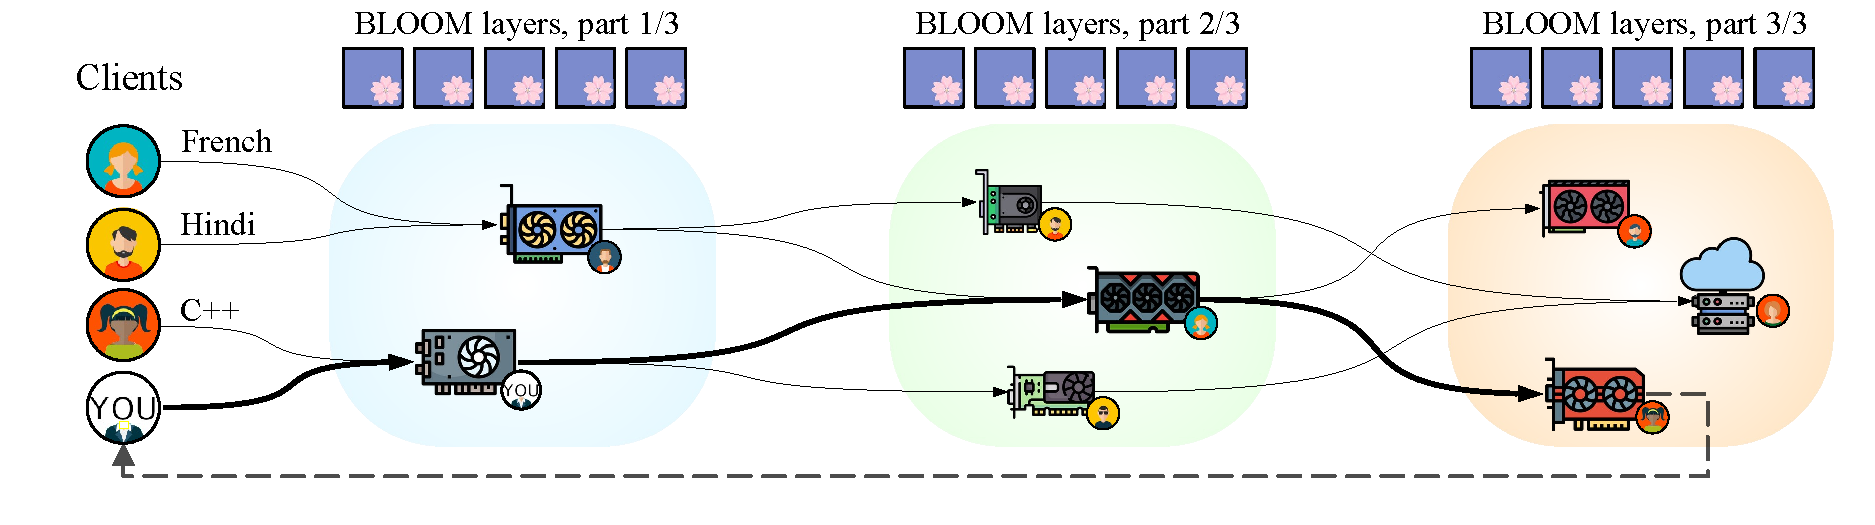
\includegraphics[width=\linewidth]{resources/bloom_swarm_eyeless.pdf} %
    \vspace{-20px}\caption{A high-level overview of our system design. Servers store pretrained LLM layers and temporarily hold attention caches for inferencing. Clients hold embedding layers and learned prompts/adapters (if used).
    Arrows denote temporary chains formed for inference.}
    \vspace{-15px}
    \label{fig:algorithm}
\end{figure*}

In this work, we search for a more cost-effective way of running pretrained LLMs in their main use cases: inference, in-context learning, and fine-tuning. We analyze latency and throughput for these use cases and determine which factors become dominant for very large models. Notably, for models with over 50B parameters, communicating activations over a slow network can be faster than swapping layers from local RAM or SSD. Based on these observations, it should be possible to run LLMs cost-effectively by pooling together commodity hardware over the Internet.


However, existing LM algorithms are not designed to run inference with unreliable devices or high-latency networks. To bridge this gap, we formulate a novel algorithm for fault-tolerant distributed autoregressive inference of very large models. Using dual attention caches, this algorithm can quickly recover from a failed server and reassign the load to one or more replacement servers. Finally, to make sure that there are enough servers for every part of the model, we develop a decentralzied load-balancing algorithm that assigns transformer blocks to every server to maximize the total system throughput. The fully decentralized nature of these protocols allows participants to add or remove their devices at any point, making optimal use of GPU idle time.

We summarize the main contributions of this work as such:
\begin{itemize}
    \item We analyze the problem of cost-efficient LLM inference and propose a novel algorithm that can inference large (50B+) language models on distributed unreliable devices. To the best of our knowledge, this is the first algorithm that can inference LLMs with 50B+ parameters in this setup.
    \item Using this algorithm, we develop \textsc{Petals}~--- a decentralized system for inferencing and fine-tuning LLMs over the Internet. The system allows users to run inference and fine-tuning over a swarm of unreliable devices with the same correctness guarantees as when running locally. The system runs persistently with the help of volunteers.
    \item We benchmark the performance of the proposed algorithms on Llama 2 (70B)~\citep{llama2} and BLOOM (176B)~\citep{bloom}. We run experiments in controlled conditions, with simulated network latency and server failures, and in the actual geo-distributed system spanning two continents. With realistic network speeds, our distributed algorithms perform autoregressive generation ${\geq}10\times$ faster than local offloading.
\end{itemize}

